\PassOptionsToPackage{unicode=true}{hyperref} % options for packages loaded elsewhere
\PassOptionsToPackage{hyphens}{url}
%
\documentclass[]{article}
\usepackage{lmodern}
\usepackage{amssymb,amsmath}
\usepackage{ifxetex,ifluatex}
\usepackage{fixltx2e} % provides \textsubscript
\ifnum 0\ifxetex 1\fi\ifluatex 1\fi=0 % if pdftex
  \usepackage[T1]{fontenc}
  \usepackage[utf8]{inputenc}
  \usepackage{textcomp} % provides euro and other symbols
\else % if luatex or xelatex
  \usepackage{unicode-math}
  \defaultfontfeatures{Ligatures=TeX,Scale=MatchLowercase}
\fi
% use upquote if available, for straight quotes in verbatim environments
\IfFileExists{upquote.sty}{\usepackage{upquote}}{}
% use microtype if available
\IfFileExists{microtype.sty}{%
\usepackage[]{microtype}
\UseMicrotypeSet[protrusion]{basicmath} % disable protrusion for tt fonts
}{}
\IfFileExists{parskip.sty}{%
\usepackage{parskip}
}{% else
\setlength{\parindent}{0pt}
\setlength{\parskip}{6pt plus 2pt minus 1pt}
}
\usepackage{hyperref}
\hypersetup{
            pdfborder={0 0 0},
            breaklinks=true}
\urlstyle{same}  % don't use monospace font for urls
\usepackage[margin=1in]{geometry}
\usepackage{graphicx,grffile}
\makeatletter
\def\maxwidth{\ifdim\Gin@nat@width>\linewidth\linewidth\else\Gin@nat@width\fi}
\def\maxheight{\ifdim\Gin@nat@height>\textheight\textheight\else\Gin@nat@height\fi}
\makeatother
% Scale images if necessary, so that they will not overflow the page
% margins by default, and it is still possible to overwrite the defaults
% using explicit options in \includegraphics[width, height, ...]{}
\setkeys{Gin}{width=\maxwidth,height=\maxheight,keepaspectratio}
\setlength{\emergencystretch}{3em}  % prevent overfull lines
\providecommand{\tightlist}{%
  \setlength{\itemsep}{0pt}\setlength{\parskip}{0pt}}
\setcounter{secnumdepth}{0}
% Redefines (sub)paragraphs to behave more like sections
\ifx\paragraph\undefined\else
\let\oldparagraph\paragraph
\renewcommand{\paragraph}[1]{\oldparagraph{#1}\mbox{}}
\fi
\ifx\subparagraph\undefined\else
\let\oldsubparagraph\subparagraph
\renewcommand{\subparagraph}[1]{\oldsubparagraph{#1}\mbox{}}
\fi

% set default figure placement to htbp
\makeatletter
\def\fps@figure{htbp}
\makeatother


\author{}
\date{\vspace{-2.5em}}

\begin{document}

\hypertarget{supporting-information-for-a-standardized-effect-size-for-evaluating-the-strength-of-phylogenetic-signal-and-why-lambda-is-not-appropriate}{%
\section{Supporting Information for: A Standardized Effect Size for
Evaluating the Strength of Phylogenetic Signal, and Why Lambda is not
Appropriate}\label{supporting-information-for-a-standardized-effect-size-for-evaluating-the-strength-of-phylogenetic-signal-and-why-lambda-is-not-appropriate}}

Here we provide additional supporting information referenced in the main
document: additional analyses, and simulation results across a wider set
of input conditions.

\hypertarget{simulations-on-differently-shaped-phylogenies}{%
\subsection{Simulations on differently shaped
phylogenies}\label{simulations-on-differently-shaped-phylogenies}}

In addition to using pure-birth phylogenies, we explored the effect of
tree shape on our findings using both balanced and pectinate trees. As
before, simulations were conducted on a range of tree sizes
(\(n=2^5 - 2^{10}\)), and across a range of input levels of phylogenetic
signal (\(\lambda_{in} = 0.0 \to 1.0\); in 21 intervals of 0.05 units).
For each \(n\) and \(\lambda_{in}\) combination, 50 replicates of a
continuous trait were simulated using a Brownian motion model of
evolution. Using these, we estimated the degree of phylogenetic signal
using \(\lambda\). \hfill\break

\emph{Results}. As found with pure-birth phylogenies, estimates of
\(\lambda\) varied most dramatically in simulations with fewer species
and at intermediate values of lambda (Fig. S1, S2). Pectinate trees
showed an interesting tendency to underestimate \(\lambda\) across input
values. Most dramatically, some simulations on the largest pectinate
phylogeny (\(n = 1024\)) estimated \(\lambda = 0\) for input values as
high as 0.5 (Fig. S2).

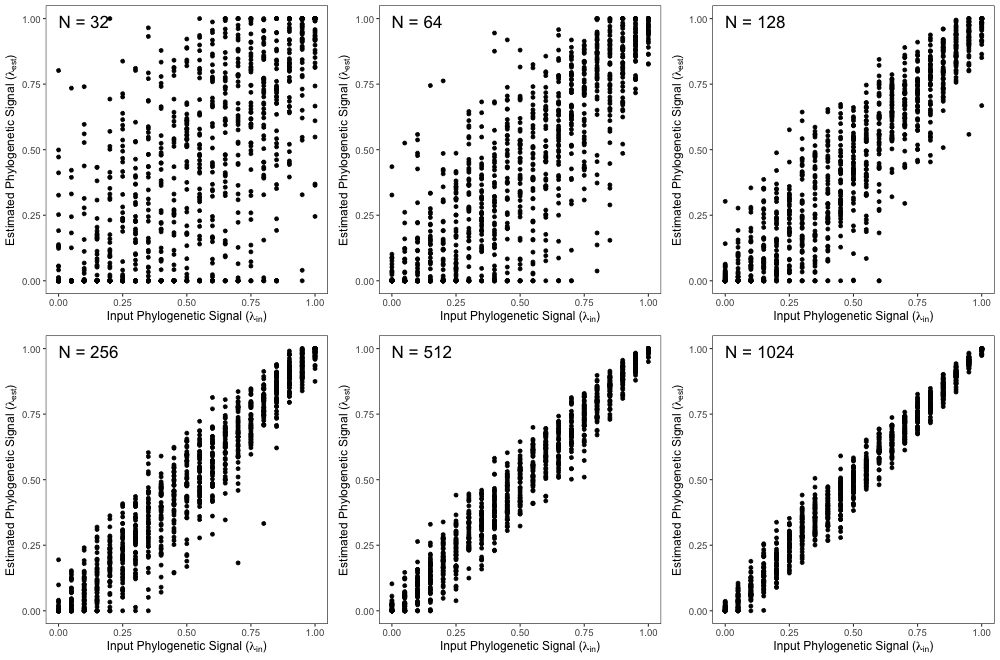
\includegraphics[width=0.95\linewidth]{FigS1}

\textbf{Figure S1}. Accuracy of Pagel's lambda estimations across known
lambda inputs on various tree sizes. Results obtained using balanced
trees. \hfill\break

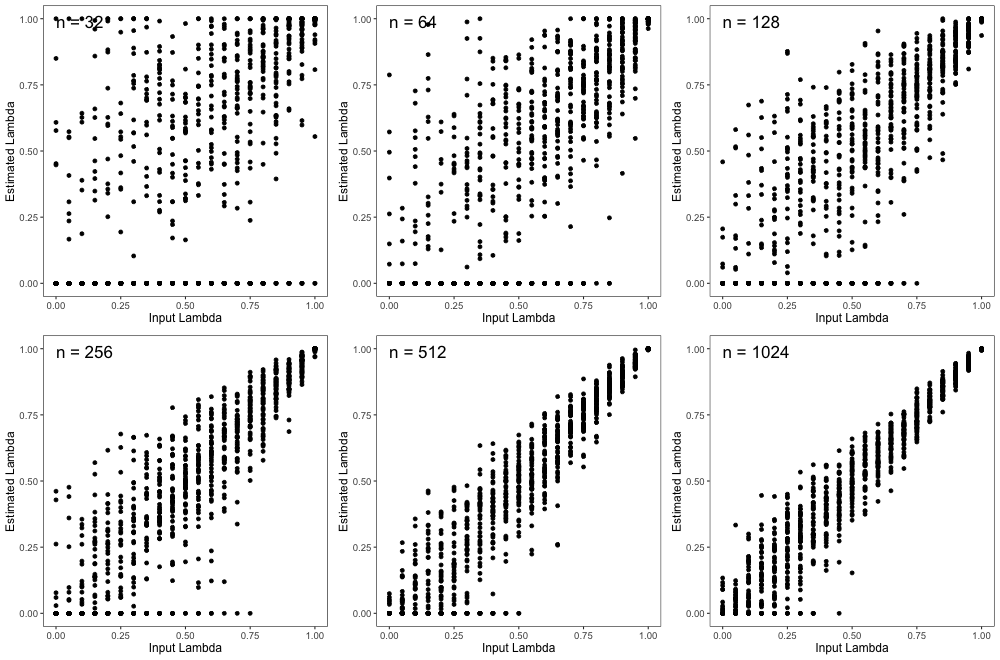
\includegraphics[width=0.95\linewidth]{FigS2}

\textbf{Figure S2}. Accuracy of Pagel's lambda estimations across known
lambda inputs on various tree sizes. Results obtained using pectinate
trees.

\hypertarget{simulations-of-phylogenetic-regression-and-anova}{%
\subsection{Simulations of phylogenetic regression and
ANOVA}\label{simulations-of-phylogenetic-regression-and-anova}}

We analyzed the precision of parameter estimation when parameters were
obtained in phylogenetic regression and ANOVA. This involved simulations
of dependent variables with \(\lambda\) values ranging from 0 to 1 (21
intervals of 0.05 units) across pure-birth trees (\(n=2^5 - 2^{10}\)).
For each \(\lambda\) input value, independent variables were then
generated with a known relationship to the simulated dependent variable
(\(\beta = 0, 0.25, 0.5, 0.75, 1.0\)), from which \(\lambda\) was then
estimated.

\emph{Results} As with the results from the regression analyses in the
main text, we found poor precision of \(\lambda\) estimation in smaller
trees and at intermediate levels of phylogenetic signal with
phylogenetic ANOVA (Fig. S3). Slope was reliably estimated across tree
sizes and known \(\lambda\) values (Fig. S4).

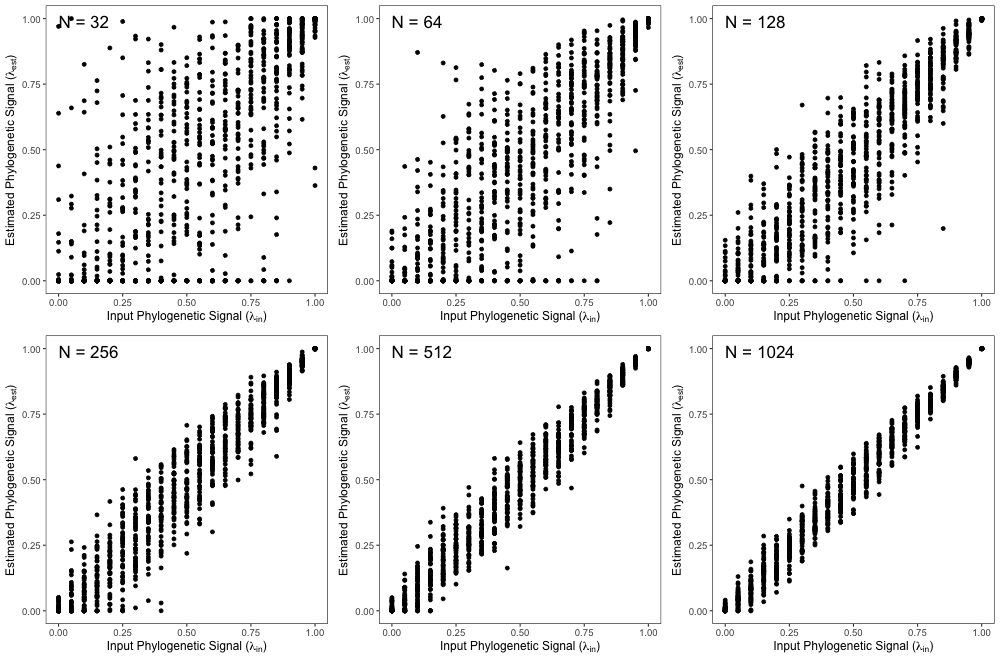
\includegraphics[width=0.95\linewidth]{FigS3}

\textbf{Figure S3}. Precision of Pagel's \(\lambda\) when incorporated
in phylogenetic ANOVA. Results are from input \(\beta\) values of
\(0.5\). \hfill\break

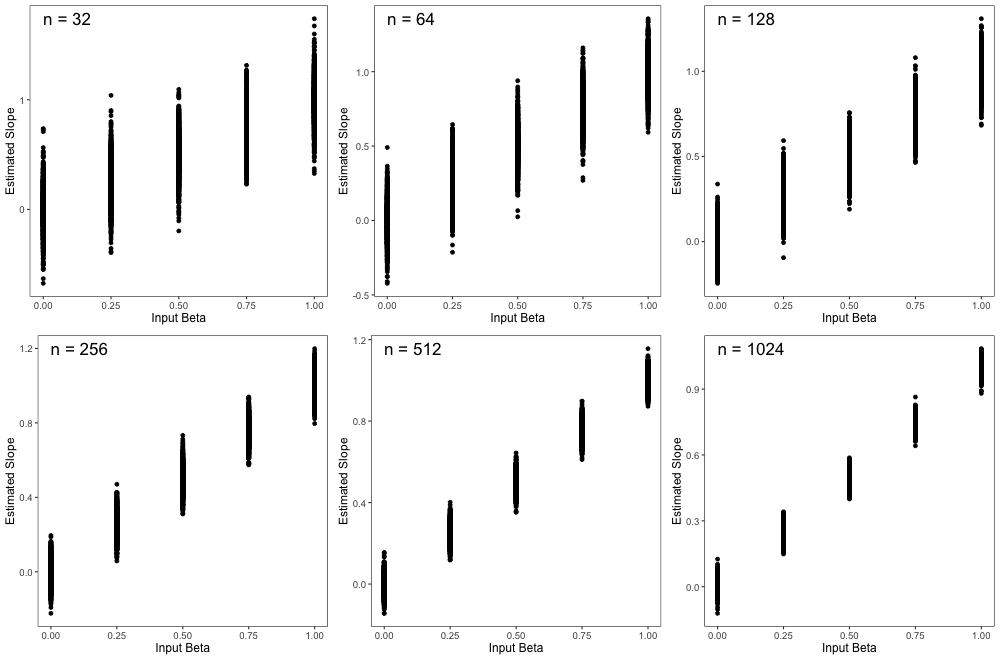
\includegraphics[width=0.95\linewidth]{FigS4}

\textbf{Figure S4}. Precision of slope estimates across known input
\(\beta\) values of phylogenetic regression. Results shown include all
input \(\lambda\) values.

\hypertarget{effect-sizes-of-pagels-lambda-z_lambda-and-kappa-z_kappa}{%
\subsection{\texorpdfstring{Effect Sizes of Pagel's Lambda
(\(Z_\lambda\)) and Kappa
(\(Z_{\kappa}\))}{Effect Sizes of Pagel's Lambda (Z\_\textbackslash{}lambda) and Kappa (Z\_\{\textbackslash{}kappa\})}}\label{effect-sizes-of-pagels-lambda-z_lambda-and-kappa-z_kappa}}

We proposed the use of effect sizes (Z-scores) as a measure of the
strength of phylogenetic signal. These were obtained from summary
parameters of phylogenetic signal: \(\lambda\) and \(\kappa\). The
precision of effect sizes \(Z_\lambda\) and \(Z_{\kappa}\) are
summarized in the main text, primarily for simulations where \(n=32\).
Here we present results from additional simulations.

\emph{Results} Effect sizes for Pagel's \(\lambda\) (\(Z_\lambda\))
scale nonlinearly with input levels of phylogenetic signal, and this
pattern is consistent across all tree sizes examined (Figure S5).
Further, the precision of \(Z_\lambda\) varied widely across input
levels of phylogenetic signal, with decidely greater variation (less
precision) at stronger input levels of phylogenetic signal (Figure S5).
By contrast, effect sizes for \(\kappa\) (\(Z_{\kappa}\)) displayed a
linear increase with increasing input levels of phylogenetic signal,
which remained consistent across all tree sizes examined (Figure S6).
Additionally, the precision of \(Z_{\kappa}\) remained constant across
input levels of phylogenetic signal (Figure S6). Together these results
imply that \(Z_{\kappa}\) is a more reliable estimate of the strength of
phylogenetic signal.

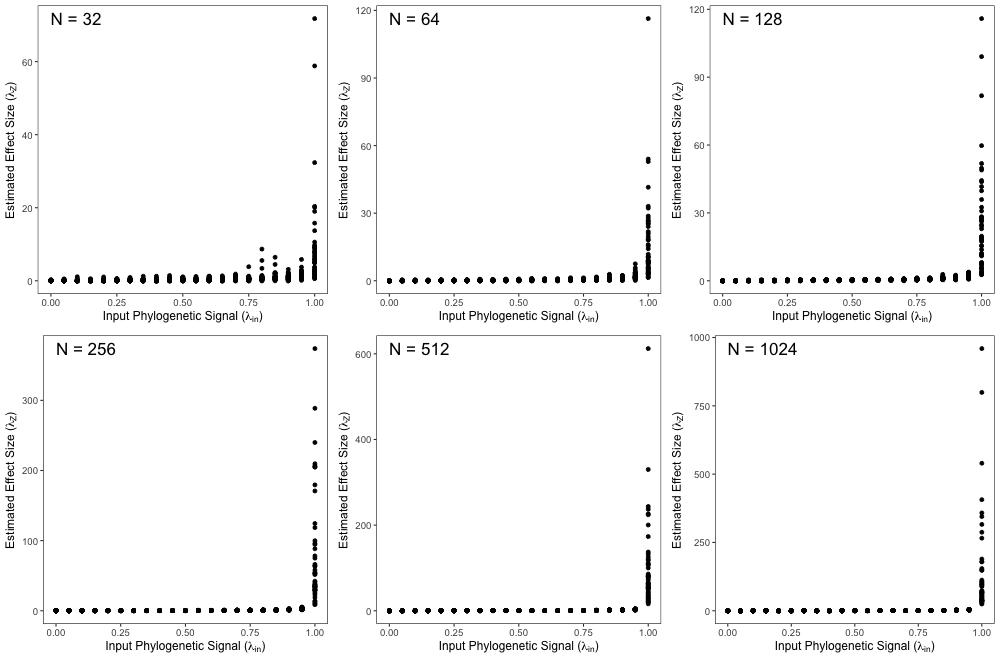
\includegraphics[width=0.95\linewidth]{FigS5}

\textbf{Figure S5}. Variation in effect size (Z score) of Pagel's
\(\lambda\) across input \(\lambda\) values on various tree sizes.
\hfill\break

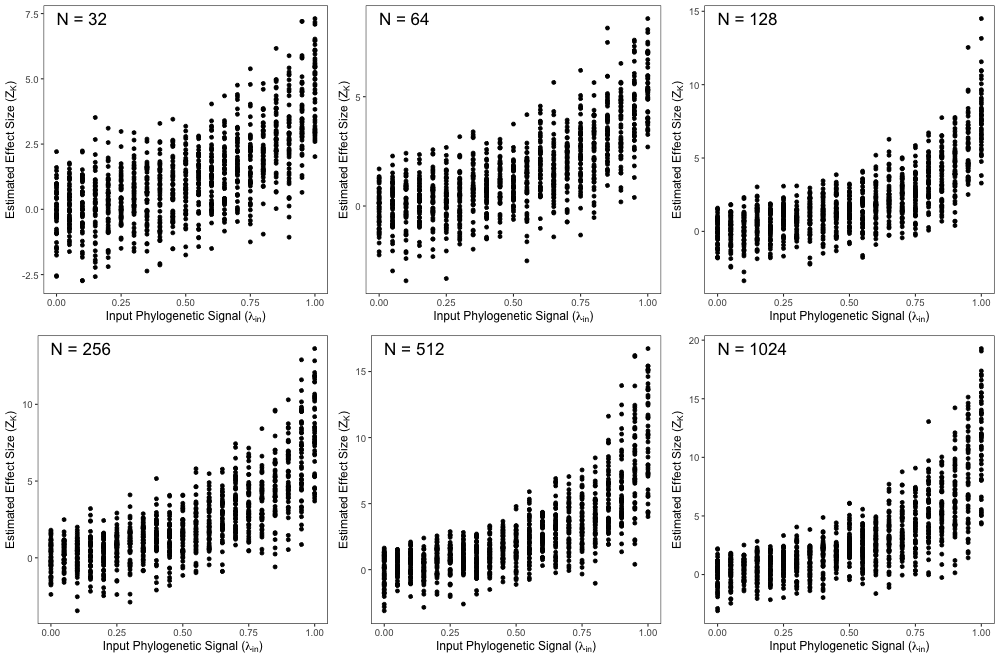
\includegraphics[width=0.95\linewidth]{FigS6}

\textbf{Figure S6}. Variation in effect size (Z score) of \(\kappa\)
across input \(\lambda\) values on various tree sizes. \hfill\break

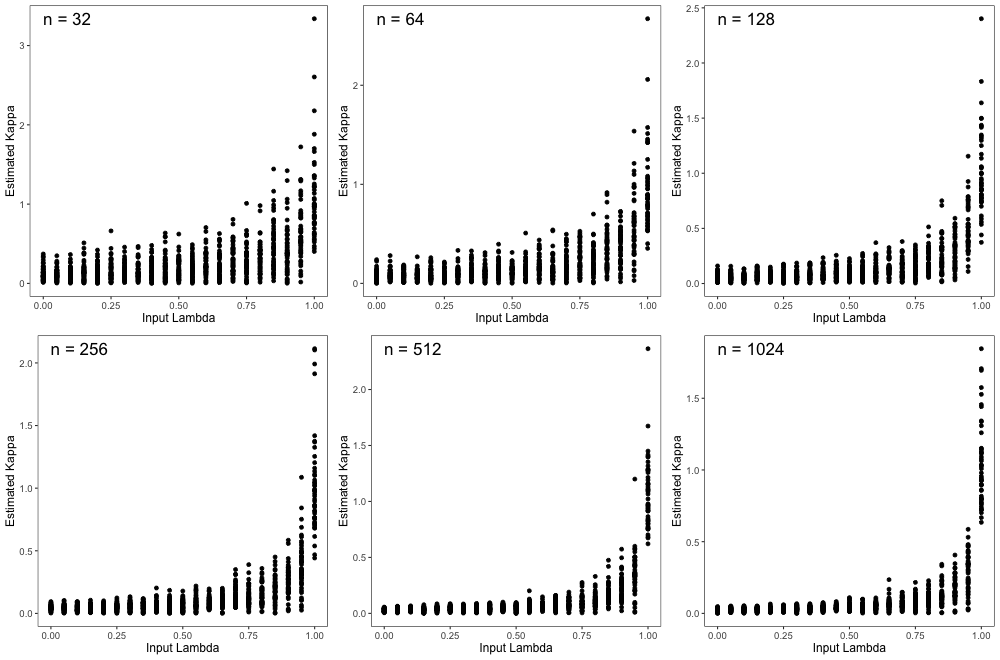
\includegraphics[width=0.95\linewidth]{FigS7}

\textbf{Figure S7}. Estimates of phylogenetic signal using \(\kappa\)
across known lambda inputs on various tree sizes. Plot shows that while
\(\kappa\) increases with increasing phylogenetic signal, the precision
of this estimate also varies. Thus, conversion to a standardized effect
size (\(Z_{\kappa}\)) is preferred.

\end{document}
